\chapter{Test on EEG measurements}
Through this chapter a modification of the main algorithm will be described such that the main algorithm can handled real EEG measurements. 

For verification of the results the MSE values achieved from the EEG measurements will be compared to MSE values achieved from the use of ICA, cf. appendix. This would include some preprocessing of the used EEG measurements.

At last, from the observed results of the comparison a conclusion will close this chapter.

\section{Data Description}
The data set of interest in this chapter consist of real EEG scalp measurements which has been provided for this thesis. The EEG scalp measurements are achieved from a experiment with a EEG cap where the test person was closing and opening his/her eyes. For the experiment a cap with $M = 27$ sensors has been used to measure the mixing of sources over a period of XX seconds. The data set then only consist of the measurement matrix $\mathbf{Y} \in \mathbb{R}$ and not the source matrix and mixing matrix as the data sets described in chapter \ref{ch:implementation}.



\begin{itemize}
\item S1\_Cclean is clean data for the forst subject for closed-yeys condition
\item 27 channels with names and position in EEG.chanlocs structure 
\item Preprocessed: The data is bandpass filtered between 1 and 40 Hz. Then decomposed by ICA and the independent components related to eye activity was removed.
\item S1\_Cclean is divided into 144 segments (0ne second long), with 27 sensor and 515 samples each (144 x 27 x 515).  X is found from ICA and is of size 144 x 27 x 513. X\_nonzero is X from ICA consisting of only active sources (144 x k x 513) where k is different for each segment (k is 144 long). The nonzero values if found from a tolerance of 10E-03 and -10E-03 such that at box around zero is equal to zero while the rests keep their original values (k). This is done by look at the average of one row and compared to the tolerance.
\end{itemize}
\section{Implementing of Baseline Algorithm}
\begin{itemize}
\item Removing Cov-DL and replace it with a random A
\item M is known but not N(k)
\end{itemize}

\section{Test on EEG Data Set}
To investigate the performance of the main algorithm on real EEG measurements a comparison which the ICA algorithm will be conducted. For this comparison three cases will be investigated: $M = N$, $M < N$ with a third of the sensors removed, $M << N$ with every second sensor removed. For all three cases the MSE values of the main algorithm will be compared to the same MSE values from the ICA algorithm obtained when $M=N$.

First, a description of how the MSE values from the ICA algorithm is found from the EEG measurement data set.
The ICA algorithm take the measurement matrix $\mathbf{Y}_s \in \mathbb{R}^{M \times L_s}$ for each segment $s$ as input and produced a source matrix $\mathbf{X}_s \in \mathbb{R}^{N \times L_s}$ for each segment $s$. Remember that the number of sensors equal the number of sources, $M = N$, but as mentioned in chapter XX, the case of interest are the active sources $k$, and by that $N = k$. 
For each source matrix $\mathbf{X}_s$ one need to find the $k$ active sources but it is not as easy as one may have though. Each entries of the sources matrix are to small to be detected from being active (non-zero) or being non-active (zeros).
Instead a tolerance is defined for which values less will be determined as zeros. As the source matrices have positive and negative values a tolerance interval, an interval around zero, must be made. Let the tolerance be defined as tol = $[10E-03, -10E-03]$ where values inside this interval is set equal to zero.
A problem occur in form of the stationarity of the sources as described in the motivation chapter \ref{ch:} sources are stationary if you look at small enough interval. For one second interval this is not the case with our EEG measurements and one can therefore not have a entire row (source) which laid the tolerance interval. One could decrease the length of the segments but one must also take in mind that smaller segments lead to more segments and therefore a higher computational complexity. Instead an average is introduced. For each rows (the sources) of each segments will be average such that one source is resembled by one average value. This average value will then be compared to the interval. If the value laid inside the tolerance interval, the whole row will be set equal to zero. The sources in each segments equal to zero are removed and the source matrix will now be of size $\mathbf{X}_s \in \mathbb{R}^{k \times L_s}$.

As mentioned only the sensors $M$ is known from the EEG measurement data sets but with the source matrices achieved from the ICA algorithm $k$ is now known for each segment. One now have all the information need to used the main algorithm on the EEG measurement data sets. 

Before any tests can be perform the localization of the sources obtain from the main algorithm must be replaced as the ICA algorithm do not localize the sources at the correct localization. For the replacement, the mse of one row from the ICA source matrix is computed with all rows of the source matrix from the main algorithm. Then the minimum is taken of all the mse values from the row of interest. The row from the main algorithm which lead to minimum MSE with the row from ICA must be the same source. The source from the main algorithm is then moved to a new source matrix where it is placed in the index that the row from ICA have. The source that was moved is then removed from the original source matrix from the main algorithm. This will be done until all rows of ICA have been compared to the rows of main. For the last replacement only one row is left from the main algorithm this could lead to some misplacement. 


\subsection{Case 0, $M = N$}
ICA is applied on $\mathbf{Y}_s$ specified by $M\_ = 27$ and $L_s = 516$. 
The main algorithm is applied on $\mathbf{Y}_s$ without any reduction hence specified by $M = 27$ and $L_s = 516$, given $\hat{\mathbf{A}}_{\text{fix}}$ and $N = k$ provided from ICA.
Figure \ref{fig:M=N_1} show $\text{MSE}\left(\hat{\mathbf{X}}_{\text{main}},\hat{\mathbf{X}}_{\text{ICA}}\right)$ for all segments $s$. 
Figure \ref{fig:M=N_1_2} show the same plot but the y-axis is specified to the interval $[-10,50]$ for better visualization.
Furthermore, the MSE tolerance $= 5$ is visualized, indicting for each segment whether the estimate $\hat{\mathbf{X}}_{\text{main}}$ is sufficiency close to $\hat{\mathbf{X}}_{\text{ICA}}$. 
For a majority of the segments the MSE lies under the tolerance, but single outliers appears for which the MSE of the segment is significantly increased. Taking the average over all segments the average achieved MSE is $5.17$.    
\begin{figure}[H]
\begin{widepage}
    \begin{minipage}[t]{.45\textwidth}
		\centering
		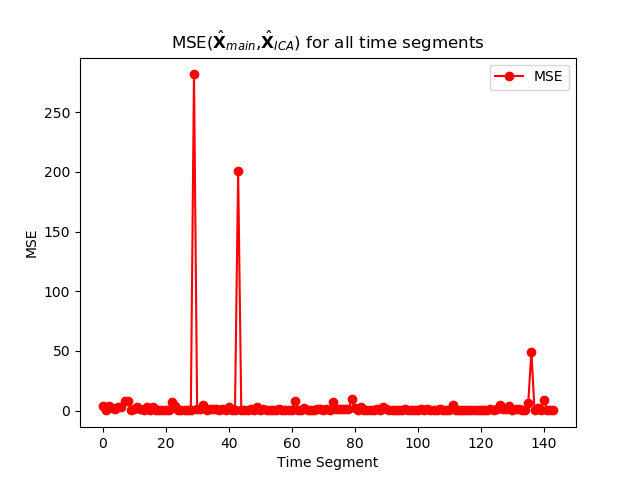
\includegraphics[width=1\linewidth]{figures/ch_7/resultat/average_mse_none_removed_ica}
	\caption{$\text{MSE} \left(\hat{\mathbf{X}}_{\text{main}}, \hat{\mathbf{X}}_{\text{ICA}}\right)$ for all $n_{\text{seg}} = $ 144 segments.}
	\label{fig:M=N_1}
    \end{minipage} 
    \hspace{0.5cm}
    \begin{minipage}[t]{.45\textwidth}
        \centering
		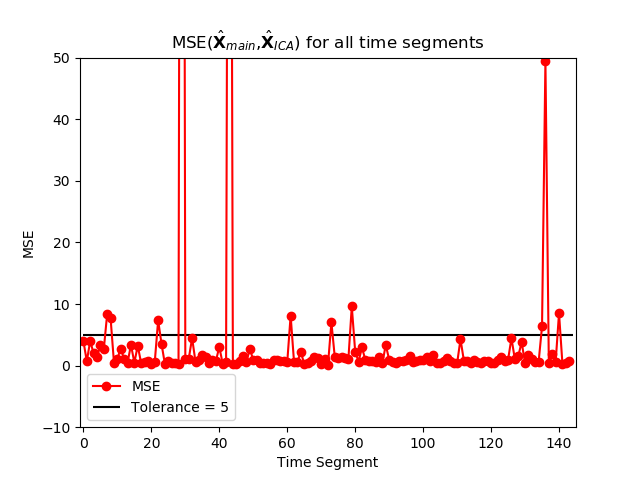
\includegraphics[width=1\linewidth]{figures/ch_7/resultat/average_mse_none_removed_ica_zoom.png}
	\caption{$\text{MSE} \left(\hat{\mathbf{X}}_{\text{main}}, \hat{\mathbf{X}}_{\text{ICA}}\right)$ for all $n_{\text{seg}} = $ 144 segments. Visualized only for the y-axis interval $[-10, 50]$ for better visualization.}
	\label{fig:M=N_1_2}
    \end{minipage}
\end{widepage}
\end{figure}
\noindent
To investigate the behavior of a single segment figure \ref{fig:M=N_2} show the MSE value computed for each row of the two estimates of a specific segment. 
That is MSE$(\hat{\mathbf{X}}_{\text{main}_{i}}$, $\hat{\mathbf{X}}_{\text{ICA}_{i}})$ for every row $i = 1, \dots, k$ in time segment $s = 5$. 
Additionally figure \ref{fig:M=N_3} show and compare the corresponding estimates for four random chosen sources. 
This allows for visual comparison of the estimates relative to the corresponding MSE value seen in figure \ref{fig:M=N_2}. 
Note that for better visual comparison each visualized row of $\hat{\mathbf{X}}_{\text{ICA}}$ is scaled with respect to the max value of the corresponding row in $\hat{\mathbf{X}}_{\text{main}}$.
From figure \ref{fig:M=N_2} it is seen that the estimate of each source result in a relative low MSE. This indicates that the main algorithm has managed to estimate the same source as the ICA algorithm. 
In contradiction to this, figure \ref{fig:M=N_3} do not confirm that the estimates are close, as generally the two signals does not follow the same trend.   
\begin{figure}[H]
\begin{widepage}
    \begin{minipage}[t]{.45\textwidth}
\centering
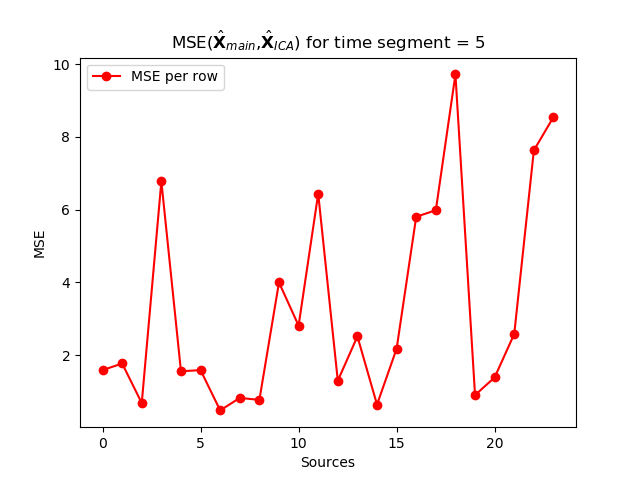
\includegraphics[width=1\linewidth]{figures/ch_7/resultat/mse_none_removed_ica_timeseg5.png}
\caption{MSE$\left(\hat{\mathbf{X}}_{\text{main}_{i}},\hat{\mathbf{X}}_{\text{ICA}_{i}}\right)$ for every row $i = 1, \dots, k$ in time segment $s=5$.}
\label{fig:M=N_2}
\end{minipage} 
\hspace{0.5cm}
\begin{minipage}[t]{.45\textwidth}
\centering
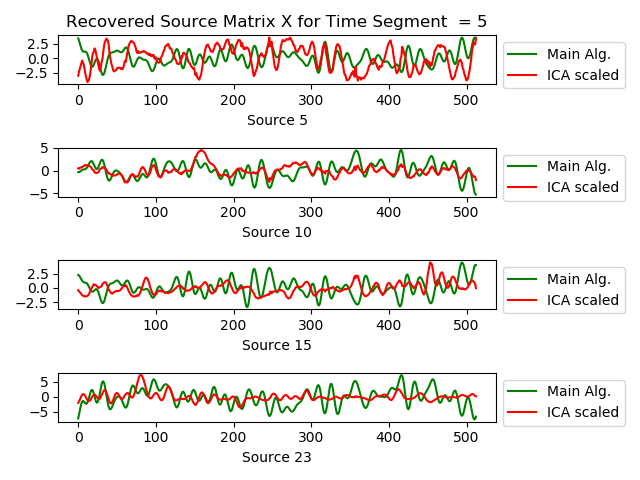
\includegraphics[width=1\linewidth]{figures/ch_7/resultat/EEG_none_removed_scaled_timeseg5S1_CClean.png}
\caption{Figure comparing four random chosen rows from $\hat{\mathbf{X}}_{\text{main}}$ and $\hat{\mathbf{X}}_{\text{ICA}}$ from time segment $s = 5$ with $M = N$ and $k=23$. Note $\hat{\mathbf{X}}_{\text{ICA}}$ is scaled for better visualization.}
	\label{fig:M=N_3}
    \end{minipage}
\end{widepage}
\end{figure}
\noindent
The test is repeated for every data set, and the results are summarized in table \ref{tab:case_0}. 
In general a low MSE is achieved in average over all segments of one data set relative to the tolerance.
And the corresponding percentage is likewise relative high, with an average at $83\%$. 
A single result is seen to deviate from the tendency, which is the data set of test subject 3 with closed eyes. 
Here a significant high average MSE value is found, indicating a majority of the segment has resulted in a significantly high MSE, while a percentage of $63\%$ was below the tolerance. 
In chapter \ref{ch:implementation} it is found that the main algorithm was capable of providing an almost exact estimate for $M = N$ when the true $\mathbf{A}$ is provided. 
Thus, it is expected that the general performance is decreased in this case where the true $\mathbf{A}$ is unknown and $\hat{\mathbf{A}}_{\text{fix}}$ is given.

The achieved results will serve as reference when analyzing the results of the following cases where the main algorithm is applied on data set with reduced number of sensors compared to the original data set.         
\begin{table}[H]
\centering
\begin{tabular}{|c|c|c|c|c|c|c|}
\hline
\multirow{2}{*}{\textbf{\begin{tabular}[c]{@{}c@{}}Case 0 \\ $M = N$\end{tabular}}} & \multicolumn{2}{c|}{Test subject 1} & \multicolumn{2}{c|}{Test subject 2} & \multicolumn{2}{c|}{Test subject 3} \\ \cline{2-7} 
                                                                                  & Open             & Close            & Open             & Close            & Open            & Close             \\ \hline
\multicolumn{1}{|c|}{Average MSE($\hat{\mathbf{X}}_{\text{ICA}},\hat{\mathbf{X}}_{\text{main}}$)}                                               & 2.913            & 5.172            & 1.572            & 15.06            & 4.753            & 19.44           \\ \hline
\begin{tabular}[c]{@{}c@{}}Segments below \\ tolerance in \%\end{tabular}          & 91             & 92            & 98 & 61             & 87            & 63 \\ \hline
\end{tabular}
\caption{Summarized results for case 0. Test is performed on the every data set.}
\label{tab:case_0}
\end{table}	
\noindent

\subsection{Case 1, $M < N$}
The main algorithm is applied on $\mathbf{Y}_s$, where the number of sensors is reduced by one-third. 
As such the main algorithm is applied on $\mathbf{Y}_s$ specified by $M = 18$ and $L_s = 516$, given $\hat{\mathbf{A}}_{\text{fix}}$ and $N = k$ provided from ICA. 
ICA is applied on the original data set with segments $\mathbf{Y}_s$ specified by $M\_ = 27$ and $L_s = 516$.  
The viewed figures correspond to those of case 0, but for the reduced number of sources $M < N$, hence detailed figure description is omitted here.   

From figure \ref{fig:M<N_1} and \ref{fig:M<N_1_2} it is seen that a majority of the segments have MSE value close to the tolerance, but the number of outliers have increased compared to case 0.
This indicates that for an increased number of segments the main algorithm do not manage to estimate enough sources sufficiently in order to stay below the tolerance. Taking the average over all segments the average achieved MSE is $5.35$.
\begin{figure}[H]
\begin{widepage}
    \begin{minipage}[t]{.45\textwidth}
		\centering
		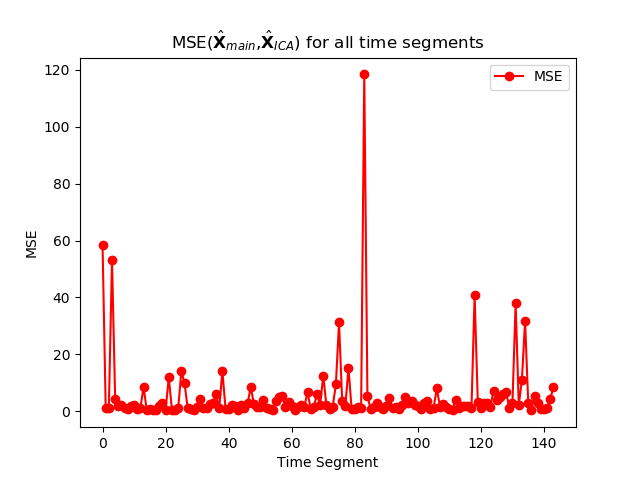
\includegraphics[width=1\linewidth]{figures/ch_7/resultat/average_mse_third_removed_ica}
	\caption{MSE$\left(\hat{\mathbf{X}}_{\text{main}},\hat{\mathbf{X}}_{\text{ICA}}\right)$ for all $n_{\text{seg}} = $ 144 segments.}
	\label{fig:M<N_1}
    \end{minipage} 
\hspace{0.5cm}
    \begin{minipage}[t]{.45\textwidth}
        \centering
		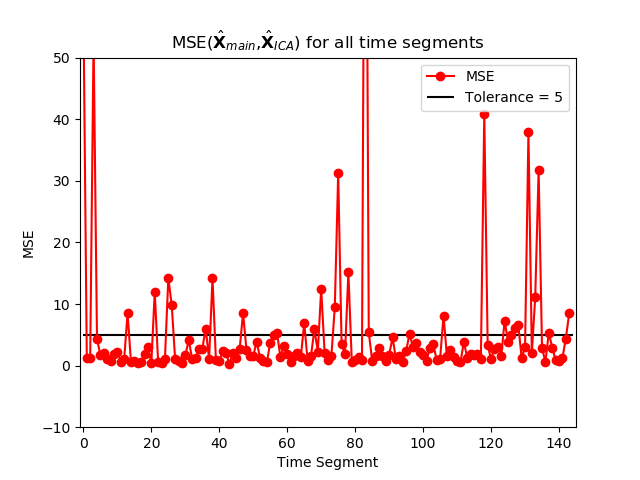
\includegraphics[width=1\linewidth]{figures/ch_7/resultat/average_mse_third_removed_ica_zoom.png}
	\caption{MSE$\left(\hat{\mathbf{X}}_{\text{main}},\hat{\mathbf{X}}_{\text{ICA}}\right)$ for all $n_{\text{seg}} = $ 144 segments. Visualized only for the y-axis interval $[-10, 50]$ for better visualization.}
	\label{fig:M<N_1_2}
    \end{minipage}
\end{widepage}
\end{figure}
\noindent 
From figure \ref{fig:M<N_2} and \ref{fig:M<N_3} showing the results of segment 5, it is seen that the MSE for each source has increased slightly compared to case 0. 
This supports the observation from figure \ref{fig:M<N_1_2}.      
\begin{figure}[H]
\begin{widepage}
    \begin{minipage}[t]{.45\textwidth}
\centering
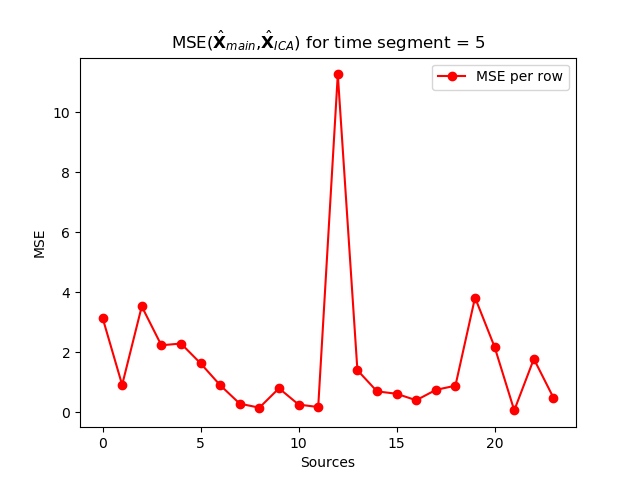
\includegraphics[width=1\linewidth]{figures/ch_7/resultat/mse_third_removed_ica_timeseg5.png}
\caption{MSE$\left(\hat{\mathbf{X}}_{\text{main}_{i}},\hat{\mathbf{X}}_{\text{ICA}_{i}}\right)$ for every row $i = 1, \dots, k$ in time segment $s=5$.}
\label{fig:M<N_2}
\end{minipage} 
\hspace{0.5cm}
\begin{minipage}[t]{.45\textwidth}
\centering
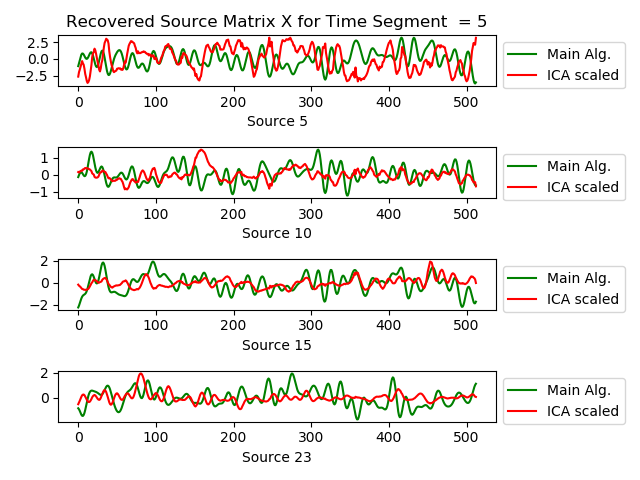
\includegraphics[width=1\linewidth]{figures/ch_7/resultat/EEG_third_removed_scaled_timeseg5S1_CClean.png}
\caption{Figure comparing four random chosen rows from $\hat{\mathbf{X}}_{\text{main}}$ and $\hat{\mathbf{X}}_{\text{ICA}}$ from time segment $s = 5$ with $M = N$ and $k=23$. Note $\hat{\mathbf{X}}_{\text{ICA}}$ is scaled for better visualization.}
	\label{fig:M<N_3}
    \end{minipage}
\end{widepage}
\end{figure}
\noindent
The test is repeated for every data set, and the results are summarized in table \ref{tab:case_1}. 
Comparing table \ref{tab:case_1} to table \ref{tab:case_0}, it is seen that the percentage of segments below the tolerance are decreasing, with the majority being close to $50\%$.
This is roughly indicating that half of the time the main algorithm do not manage to provide a sufficient estimate when $M = 2/3N$.  
Furthermore, both the average MSE and the corresponding percentages appear fluctuating relative to case 0 indicating some unreliability in the results.  
\begin{table}[H]
\centering
\begin{tabular}{|c|c|c|c|c|c|c|}
\hline
\multirow{2}{*}{\textbf{\begin{tabular}[c]{@{}c@{}}Case 1 \\ $M < N$\end{tabular}}} & \multicolumn{2}{c|}{Test subject 1} & \multicolumn{2}{c|}{Test subject 2} & \multicolumn{2}{c|}{Test subject 3} \\ \cline{2-7} 
                                                                                  & Open             & Close            & Open             & Close            & Open              & Close           \\ \hline
\multicolumn{1}{|c|}{Average MSE($\hat{\mathbf{X}}_{\text{ICA}},\hat{\mathbf{X}}_{\text{main}}$)}                                               & 9.79            & 5.351            & 13.89            & 15.13            & 6.25          & 18.21          \\ \hline
\begin{tabular}[c]{@{}c@{}}Segments below \\ tolerance in \%\end{tabular}          & 53             & 80             & 66 & 46             & 77              & 48            \\ \hline
\end{tabular}
\caption{Summarized results for case 1. Test is performed on the every data set.}
\label{tab:case_1}
\end{table}
\noindent

\subsection{Case 2, $M << N$}
The main algorithm is applied on $\mathbf{Y}_s$, where the number of sensors is reduced to half. 
As such the main algorithm is applied on $\mathbf{Y}_s$ specified by $M = 13$ and $L_s = 516$, given $\hat{\mathbf{A}}_{\text{fix}}$ and $N = k$ provided from ICA.  
ICA is applied on the original data set with segments $\mathbf{Y}_s$ specified by $M\_= 27$ and $L_s = 516$. 
The viewed figures correspond to those of case 0 and case 1, but for further reduce number of sources $M << N$, hence detailed figure description is omitted.   

From figure \ref{fig:M<<N_1} and \ref{fig:M<<N_1_2} it is seen that the MSE value for each segment is more widely scatted around the tolerance, compared to case 0 and 1. 
Outliers, where the MSE value has increased significantly, do also occur similar to case 1. 
This indicates that the performance of the main algorithm has decreased further, compared to case 1. Taking the average over all segments the average achieved MSE is $11.36$.
\begin{figure}[H]
\begin{widepage}
    \begin{minipage}[t]{.45\textwidth}
		\centering
		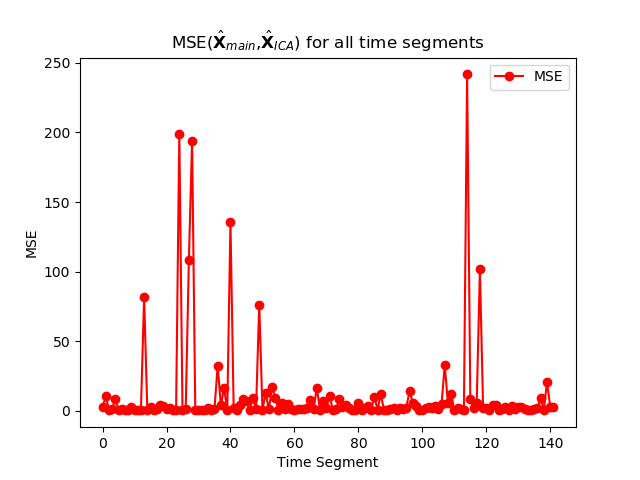
\includegraphics[width=1\linewidth]{figures/ch_7/resultat/average_mse_second_removed_ica}
	\caption{MSE$\left(\hat{\mathbf{X}}_{\text{main}},\hat{\mathbf{X}}_{\text{ICA}}\right)$ for all $n_{\text{seg}} = $ 144 segments.}
	\label{fig:M<<N_1}
    \end{minipage} 
\hspace{0.5cm}
    \begin{minipage}[t]{.45\textwidth}
        \centering
		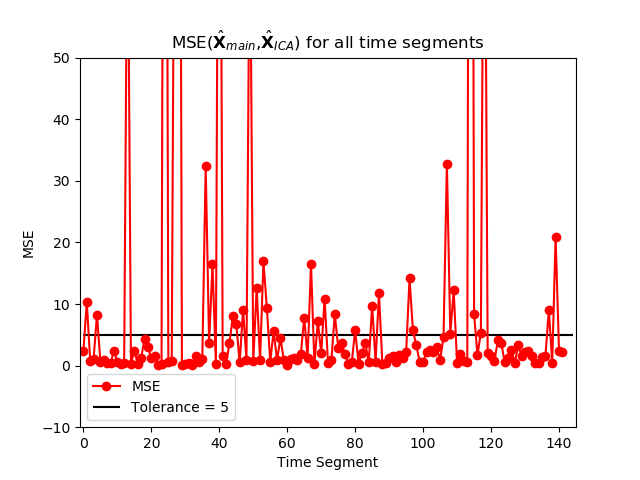
\includegraphics[width=1\linewidth]{figures/ch_7/resultat/average_mse_second_removed_ica_zoom.png}
	\caption{MSE$\left(\hat{\mathbf{X}}_{\text{main}},\hat{\mathbf{X}}_{\text{ICA}}\right)$ for all $n_{\text{seg}} = $ 144 segments. Visualized only for the y-axis interval $[-10, 50]$ for better visualization.}
	\label{fig:M<<N_1_2}
    \end{minipage}
\end{widepage}
\end{figure}
\noindent 
The above indication is supported by figure \ref{fig:M<<N_2} and \ref{fig:M<<N_3} showing an general increase in MSE. 
However, segment 5 makes a fairly good example as the majority of the sources have achieves a MSE below the tolerance of 5. 
From figure \ref{fig:M<<N_3} the increased MSE do not appear visually compared to either case 1 or case 0.        
\begin{figure}[H]
\begin{widepage}
    \begin{minipage}[t]{.49\textwidth}
\centering
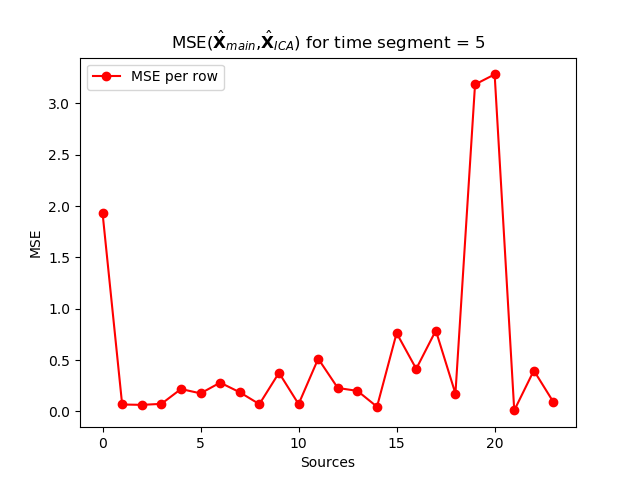
\includegraphics[width=1\linewidth]{figures/ch_7/resultat/mse_second_removed_ica_timeseg5.png}
\caption{MSE$\left(\hat{\mathbf{X}}_{\text{main}_{i}},\hat{\mathbf{X}}_{\text{ICA}_{i}}\right)$ for every row $i = 1, \dots, k$ in time segment $s = 5$.}
\label{fig:M<<N_2}
\end{minipage} 
\hspace{.5cm}
\begin{minipage}[t]{.49\textwidth}
\centering
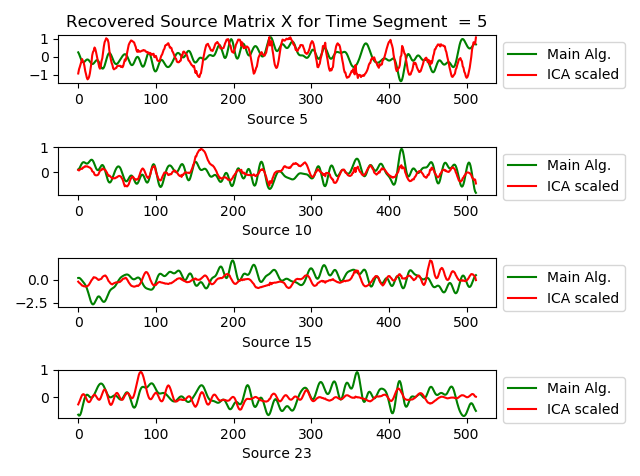
\includegraphics[width=1\linewidth]{figures/ch_7/resultat/EEG_second_removed_scaled_timeseg5S1_CClean.png}
\caption{Figure comparing four random chosen rows from $\hat{\mathbf{X}}_{\text{main}}$ and $\hat{\mathbf{X}}_{\text{ICA}}$ from time segment $s = 5$ with $M << N$ and $k=23$. Note $\hat{\mathbf{X}}_{\text{ICA}}$ is scaled for better visualization.}
	\label{fig:M<<N_3}
    \end{minipage}
\end{widepage}
\end{figure}
\noindent
The test is repeated for every data set, and the results are summarized in table \ref{tab:case_2}. Comparing table \ref{tab:case_0} to table \ref{tab:case_1} it is generally seen that the percentage of segments below the tolerance are not decreased but improved.
Though, without getting close to the tendency from case 0. 
Furthermore, the average MSE have not increased remarkably compared to case 1. 
As such the performance of the main algorithm in case 2 is in general not found to be worse than for case 1.
However, a clear improvement is not seen either.  
\begin{table}[H]
\centering
\begin{tabular}{|c|c|c|c|c|c|c|}
\hline
\multirow{2}{*}{\textbf{\begin{tabular}[c]{@{}c@{}}Case 2\\ $M << N$\end{tabular}}} & \multicolumn{2}{c|}{Test subject 1} & \multicolumn{2}{c|}{Test subject 2} & \multicolumn{2}{c|}{Test subject 3} \\ \cline{2-7} 
                                                                                  & Open             & Close            & Open             & Close            & Open             & Close            \\ \hline
\multicolumn{1}{|c|}{Average MSE($\hat{\mathbf{X}}_{\text{ICA}},\hat{\mathbf{X}}_{\text{main}}$)}                                               & 8.378            & 11.36            & 19.58            & 13.11            & 13.99           & 11.96            \\ \hline
\begin{tabular}[c]{@{}c@{}}Segments below \\ tolerance in \%\end{tabular}          & 75             & 74             & 42 & 72             & 69             & 69 \\ \hline
\end{tabular}
\caption{Summarized results for case 2. Test is performed on the every data set.}
\label{tab:case_2}
\end{table}
\noindent


\section{Conclusion}